%--------------------------------------------------------------------%
%
% Title         : Postgraduate Thesis LaTex template
% Author        : Ravi Vendra Rishika <ravi.vendra.rishika@gmail.com>
%
% Page          : Main TeX
%
% It is developed especially for postgraduate students of :
%   Department of Informatics
%   Faculty of Intelligent Electrical and Informatics Technology
%   Institut Teknologi Sepuluh Nopember (ITS)
%   Surabaya, Indonesia.
%
% This LaTex template is intended to make students easier
% to write master's degree thesis in LaTex using specific
% Department of Informatics of ITS' format.
%
%--------------------------------------------------------------------%

% One-page document class
% \documentclass[12pt, a4paper, onecolumn, oneside, final, bahasa]{report}

% Two-page document class
\documentclass[12pt, a4paper, onecolumn, twoside, final, bahasa]{book}

%--------------------------------------------------------------------%
%
% Title         : Postgraduate Thesis LaTex template
% Author        : Ravi Vendra Rishika <ravi.vendra.rishika@gmail.com>
%
% Page          : Preambule (Import Library)
%
% It is developed especially for postgraduate students of :
%   Department of Informatics
%   Faculty of Intelligent Electrical and Informatics Technology
%   Sepuluh Nopember Institute of Technology (ITS)
%   Surabaya, Indonesia.
%
% This LaTex template is intended to make students easier
% to write master's degree thesis in LaTex using specific
% Department of Informatics of ITS' format.
%
%--------------------------------------------------------------------%

\special{papersize=210mm,297mm}

% Setting margin
% \usepackage[top=3cm,bottom=2.5cm,left=3cm,right=2.5cm]{geometry}
\usepackage[top=3.5cm,bottom=3cm,inner=4cm,outer=3cm]{geometry}

\usepackage{mathptmx}

% Judul bahasa Indonesia
\usepackage[indonesian]{babel}

%Includes "References" in the table of contents
\usepackage[nottoc]{tocbibind}

\usepackage[utf8]{inputenc}
\usepackage{graphicx, titling, blindtext, sectsty, chngcntr}
\usepackage{etoolbox, titlesec, parskip, watermark, eso-pic}
\usepackage[hidelinks]{hyperref}
\usepackage[pages=some]{background}
\usepackage{setspace}
\usepackage{xcolor, ragged2e}

\usepackage{amsmath, csquotes}

% Format citation
% \usepackage[style=authoryear-ibid,backend=biber]{biblatex}
% \usepackage[backend=biber,style=numeric]{biblatex}
% \usepackage[backend=bibtex,citestyle=authoryear]{biblatex}
\usepackage{natbib}

% \usepackage[T1]{fontenc}
% \usepackage{tgbonum}

\renewcommand{\baselinestretch}{1.5}

\chapterfont{\centering \Large}
\titleformat{\chapter}[display]
  {\Large\centering\bfseries}
  {\chaptertitlename\ \thechapter}{0pt}
    {\Large\bfseries\uppercase}

\setcounter{secnumdepth}{3}

\makeatletter

\makeatother

\counterwithin{figure}{section}
\counterwithin{table}{section}


% \SetWatermarkLightness{0.9}
% \SetWatermarkText{\includegraphics[angle=-45]{src/resources/its-thesis-cover.png}

% \newcommand\BackgroundPic{
%     \put(0,0){
%         \parbox[b][\paperheight]{\paperwidth}{
%             \vfill

%             \centering
%             \includegraphics[width=\paperwidth,height=\paperheight,keepaspectratio]{src/resources/its-thesis-cover.png}
            
%             \vfill
%         }
%     }
% }

% IEEE Bibliography Style
% \bibliographystyle{abbrvnat}

% Harvard Bibliography Style
% \bibliographystyle{agsm}
\bibliographystyle{src/config/agsm-emph}

% APA Bibliography Style
% \bibliographystyle{apacite}

\setcitestyle{authoryear, open = {(}, close = {)}}

\backgroundsetup{
    scale = 1,
    color = black,
    opacity = 1.0,
    angle = 0,
    contents = {%
        
\includegraphics[width = \paperwidth, height = \paperheight]{src/resources/its-thesis-cover-without-logo.png}
    }%
}

\begin{document}
    %--------------------------------------------------------------------%
%
% Title         : Postgraduate Thesis LaTex template
% Author        : Ravi Vendra Rishika <6025211015@mhs.its.ac.id>
%
% Page          : Hyphenation (Indonesian language)
%
% It is developed especially for postgraduate students of :
%   Department of Informatics
%   Faculty of Intelligent Electrical and Informatics Technology
%   Institut Teknologi Sepuluh Nopember (ITS)
%   Surabaya, Indonesia.
%
% This LaTex template is intended to make students easier
% to write master's degree thesis in LaTex using specific
% Department of Informatics of ITS' format.
%
%--------------------------------------------------------------------%

\hyphenation {
    % English
    al-go-rithm
    a-no-ma-ly
    bro-ad-band
    % Indonesian
    a-da-lah
    ak-ti-vi-tas
    al-go-rit-ma
    % General
}


    % \AddToShipoutPicture*{\BackgroundPic}
    \BgThispage
    
    % New variables defined here
    \newcommand\titleID{TESIS MAHASISWA DEPARTEMEN TEKNIK INFORMATIKA INSTITUT TEKNOLOGI SEPULUH NOPEMBER (DALAM BAHASA INDONESIA)}
    \newcommand\titleEN{POSTGRADUATE STUDENT THESIS OF INFORMATICS DEPARTMENT OF SEPULUH NOPEMBER INSTITUTE OF TECHNOLOGY (IN ENGLISH)}

    \newcommand\authorName{Nama Mahasiswa}
    \newcommand\authorNRP{60xxxxxxxx}
    
    \newcommand\firstSupervisorName{Dosen Pembimbing ke-1 (Lengkap)}
    \newcommand\firstSupervisorNameShort{Dosen Pembimbing ke-1 (Singkat)}
    \newcommand\firstSupervisorNIP{20xxxxxxxx}
    \newcommand\firstSupervisor{
        \firstSupervisorName \\
        NIP \> : \firstSupervisorNIP
    }
    
    \newcommand\secondSupervisorName{Dosen Pembimbing ke-2 (Lengkap)}
    \newcommand\secondSupervisorNameShort{Dosen Pembimbing ke-2 (Singkat)}
    \newcommand\secondSupervisorNIP{20xxxxxxxx}
    \newcommand\secondSupervisor{
        \secondSupervisorName \\
        NIP \> : \secondSupervisorNIP
    }
    
    \newcommand\firstExaminerName{Dosen Penguji ke-1 (Lengkap)}
    \newcommand\firstExaminerNameShort{Dosen Penguji ke-1 (Singkat)}
    \newcommand\firstExaminerNIP{20xxxxxxxx}
    \newcommand\firstExaminer{
        \firstExaminerName \\
        NIP \> : \firstExaminerNIP
    }
    
    \newcommand\secondExaminerName{Dosen Penguji ke-2 (Lengkap)}
    \newcommand\secondExaminerNameShort{Dosen Penguji ke-2 (Singkat)}
    \newcommand\secondExaminerNIP{20xxxxxxxx}
    \newcommand\secondExaminer{
        \secondExaminerName \\
        NIP \> : \secondExaminerNIP
    }
    
    \newcommand\thirdExaminerName{Dosen Penguji ke-3 (Lengkap)}
    \newcommand\thirdExaminerNameShort{Dosen Penguji ke-3 (Singkat)}
    \newcommand\thirdExaminerNIP{20xxxxxxxx}
    \newcommand\thirdExaminer{
        \thirdExaminerName \\
        NIP \> : \thirdExaminerNIP
    }

    \newcommand\writingDate{8 Juni 2023} % \daymonthyeardate\today

    \newcommand\finalExamDay{-}
    \newcommand\finalExamDate{-}
    \newcommand\finalExamPlace{Online}
    
    \newcommand\postgraduateProgram{Program Magister}
    \newcommand\postgraduateCourseClass{Komputasi Berbasis Jaringan}
    \newcommand\postgraduateDepartment{Departemen Teknik Informatika}
    \newcommand\postgraduateFaculty{Fakultas Teknologi Elektro dan Informatika Cerdas}
    \newcommand\postgraduateUniversity{Institut Teknologi Sepuluh Nopember}
    \newcommand\postgraduateCity{Surabaya}
    \newcommand\postgraduateYear{\the\year{}}
    
    % Custom variable

    %Basic configuration
    \author{
        \authorName \\
        \authorNRP
    }

    % \author{
    %     \authorName \\
    %     NRP \> : \authorNRP
    % }

    \date{}

    \title{
        \titleID
    }

    \renewcommand{\contentsname}{\hfill \bfseries \large \MakeUppercase{Daftar Isi} \hfill}   
    \renewcommand{\cftaftertoctitle}{\hfill}
    \renewcommand{\listtablename}{\hfill \bfseries \large \MakeUppercase{Daftar Tabel}}
    \renewcommand{\cftafterlottitle}{\hfill}
    \renewcommand{\listfigurename}{\hfill \bfseries \large \MakeUppercase{Daftar Gambar}}
    \renewcommand{\cftafterloftitle}{\hfill}
    % \renewcommand{\listlistingsname}{\hfill \bfseries \large \MakeUppercase{Daftar Snippet Kode}}
    % \renewcommand{\cftafterloftitle}{\hfill}

    \renewcommand{\cftpartleader}{\cftdotfill{\cftdotsep}}
    \renewcommand{\cftchapleader}{\cftdotfill{\cftdotsep}}

    %--------------------------------------------------------------------%
%
% Title         : Postgraduate Thesis LaTex template
% Author        : Ravi Vendra Rishika <6025211015@mhs.its.ac.id>
%
% Page          : Cover
%
% It is developed especially for postgraduate students of :
%   Department of Informatics
%   Faculty of Intelligent Electrical and Informatics Technology
%   Institut Teknologi Sepuluh Nopember (ITS)
%   Surabaya, Indonesia.
%
% This LaTex template is intended to make students easier
% to write master's degree thesis in LaTex using specific
% Department of Informatics of ITS' format.
%
%--------------------------------------------------------------------%

\clearpage

\newgeometry{top = 1.5cm, bottom = 3.0cm, left = 3.0cm, right = 3.0cm}

\pagestyle{empty}

\begin{flushleft}
    \color{white}

    \begin{figure}[h]
        \flushleft \raggedright
        
\includegraphics[width = 3.5cm, height = 3.5cm]{src/resources/its-logo.png}
    \end{figure}

    \vspace{4.0cm}

    {\fontfamily{lmss} \selectfont \large \bfseries \MakeUppercase
        IF185301 TESIS - PROPOSAL
    }

    \vspace{1.5cm}

    {\fontfamily{lmss} \selectfont \Large \bfseries \MakeUppercase
        {\thetitle}
    }

    \vspace{1.5cm}

    \begin{singlespace}
   	    {\fontfamily{lmss} \selectfont \large \bfseries \MakeUppercase
   	        {\theauthor}
        }
    \end{singlespace}

    \vspace{1.5cm}

    \begin{singlespace}
   	    {\fontfamily{lmss} \selectfont \normalsize \bfseries
   	        Dosen Pembimbing: \\
                {\firstSupervisorName} \\
                {\secondSupervisorName}
        }
    \end{singlespace}

    \vspace{1.5cm}

    \begin{singlespace}
   	    {\fontfamily{lmss} \selectfont
            \normalsize \bfseries \MakeUppercase {
                % {\postgraduateProgram} \\
                % Rumpun Mata Kuliah {\postgraduateCourseClass} \\
                {\postgraduateDepartment} \\
                {\postgraduateFaculty} \\
                {\postgraduateUniversity} \\
                % {\postgraduateCity} \\
                {\postgraduateYear}
            }
        }
    \end{singlespace}

\end{flushleft}

\restoregeometry

\clearpage

    %--------------------------------------------------------------------%
%
% Title         : Postgraduate Thesis LaTex template
% Author        : Ravi Vendra Rishika <6025211015@mhs.its.ac.id>
%
% Page          : Blank Page
%
% It is developed especially for postgraduate students of :
%   Department of Informatics
%   Faculty of Intelligent Electrical and Informatics Technology
%   Institut Teknologi Sepuluh Nopember (ITS)
%   Surabaya, Indonesia.
%
% This LaTex template is intended to make students easier
% to write master's degree thesis in LaTex using specific
% Department of Informatics of ITS' format.
%
%--------------------------------------------------------------------%

\clearpage

\pagestyle{empty}

\begin{center}
    \smallskip

    \normalsize \normalfont

    \topskip 0pt

    \vspace*{\fill}
\end{center}

\clearpage


    \pagestyle{plain}
    \pagenumbering{roman}
    \setcounter{page}{1}
    
    %--------------------------------------------------------------------%
%
% Title         : Postgraduate Thesis LaTex template
% Author        : Ravi Vendra Rishika <6025211015@mhs.its.ac.id>
%
% Page          : Approval
%
% It is developed especially for postgraduate students of :
%   Department of Informatics
%   Faculty of Intelligent Electrical and Informatics Technology
%   Institut Teknologi Sepuluh Nopember (ITS)
%   Surabaya, Indonesia.
%
% This LaTex template is intended to make students easier
% to write master's degree thesis in LaTex using specific
% Department of Informatics of ITS' format.
%
%--------------------------------------------------------------------%

\clearpage

\addcontentsline{toc}{chapter}{Lembar Pengesahan}

\newgeometry{top = 3.50cm, bottom = 3.00cm, inner = 2.75cm, outer = 2.50cm}

\begin{center}
    \smallskip

    \large \MakeUppercase{
        \textbf{Lembar Pengesahan \\
        Proposal Tesis}
    }

    \normalsize

    \begin{flushleft}
        \setlength{\tabcolsep}{5pt}
        \begin{tabular}{p{0.15\linewidth} p{0.85\linewidth}}
            Judul       & : {\thetitle} \\
            Mahasiswa   & : {\authorName} \\
            NRP         & : {\authorNRP}
        \end{tabular}
    \end{flushleft}

    \vspace{10pt}

    \normalsize
    Telah diseminarkan pada,

    \begin{flushleft}
        \setlength{\tabcolsep}{5pt}
        \begin{tabular}{p{0.15\linewidth} p{0.85\linewidth}}
            Hari        & : {\finalExamDay} \\
            Tanggal     & : {\finalExamDate} \\
            Tempat      & : {\finalExamPlace}
        \end{tabular}
    \end{flushleft}

    \vspace{10pt}

    \normalsize
    Mengetahui/Menyetujui,

    \begin{flushleft}
        \setlength{\tabcolsep}{3pt}
        \begin{tabular}{p{0.47\linewidth} p{0.55\linewidth}}
            \textbf{Dosen Penguji:} & \textbf{Dosen Pembimbing:} \\
            1. & 1. \\
            & \\
            {\firstExaminerName} & {\firstSupervisorName} \\
            NIP: {\firstExaminerNIP} & NIP: {\firstSupervisorNIP} \\
            2. & 2. \\
            & \\
            {\secondExaminerName} & {\secondSupervisorName} \\
            NIP: {\secondExaminerNIP} & NIP: {\secondSupervisorNIP} \\
            3. & \\
            & \\
            {\thirdExaminerName} & \\
            NIP: {\thirdExaminerNIP} & \\
        \end{tabular}
    \end{flushleft}
\end{center}

\restoregeometry

\clearpage

    %--------------------------------------------------------------------%
%
% Title         : Postgraduate Thesis LaTex template
% Author        : Ravi Vendra Rishika <6025211015@mhs.its.ac.id>
%
% Page          : Blank for Even Page
%
% It is developed especially for postgraduate students of :
%   Department of Informatics
%   Faculty of Intelligent Electrical and Informatics Technology
%   Institut Teknologi Sepuluh Nopember (ITS)
%   Surabaya, Indonesia.
%
% This LaTex template is intended to make students easier
% to write master's degree thesis in LaTex using specific
% Department of Informatics of ITS' format.
%
%--------------------------------------------------------------------%

\clearpage

\begin{center}
    \smallskip

    \normalsize \normalfont

    \topskip 0pt

    \vspace*{\fill}

    \textit{Halaman ini sengaja dikosongkan.}

    \vspace*{\fill}
\end{center}

\clearpage


    %--------------------------------------------------------------------%
%
% Title         : Postgraduate Thesis LaTex template
% Author        : Ravi Vendra Rishika <6025211015@mhs.its.ac.id>
%
% Page          : Original Statement
%
% It is developed especially for postgraduate students of :
%   Department of Informatics
%   Faculty of Intelligent Electrical and Informatics Technology
%   Institut Teknologi Sepuluh Nopember (ITS)
%   Surabaya, Indonesia.
%
% This LaTex template is intended to make students easier
% to write master's degree thesis in LaTex using specific
% Department of Informatics of ITS' format.
%
%--------------------------------------------------------------------%

\clearpage

\addcontentsline{toc}{chapter}{Pernyataan Orisinalitas Tesis}

\chapter*{Pernyataan Orisinalitas Tesis}

\begin{center}
    \justifying \normalsize

    \setlength{\parindent}{1.5em}
    \setlength{\parskip}{0em}

    \linespread{1.5}

    Dengan ini saya menyatakan bahwa sepanjang pengetahuan saya:

    \begin{enumerate}

        \item Pengerjaan dan penulisan tesis ini dilakukan tanpa menggunakan bantuan yang tidak dibenarkan.
        \item Segala bentuk kutipan dan acuan terhadap tulisan orang lain yang digunakan di dalam penelitian ini telah disitasi dengan benar dan menyertakan sumber referensi terkait pada bagian Daftar Pustaka.
        \item Penelitian dan naskah tesis ini belum pernah diajukan di program pendidikan di perguruan tinggi manapun.
        \item Penelitian dan naskah tesis ini belum pernah dipublikasikan pada jurnal dan prosiding manapun, baik di tingkat nasional maupun internasional.

    \end{enumerate}

    Apabila ternyata di dalam naskah tesis ini dapat dibuktikan terdapat unsur-unsur \textbf{plagiasi} ataupun melanggar hal-hal di atas, saya bersedia tesis ini digugurkan dan gelar akademik yang saya peroleh (Magister) dibatalkan, serta dikenakan sanksi sesuai dengan peraturan perundang-undangan (UU No. 20 Tahun 2003, Pasal 25 Ayat 2 dan Pasal 70) dan peraturan akademik yang berlaku di {\postgraduateDepartment}, {\postgraduateFaculty} (FT-EIC), {\postgraduateUniversity} (ITS), {\postgraduateCity}, Indonesia.
    
    \begin{table}[b!]
        \centering

        \begin{tabular}{p{8cm} c}

            & {\postgraduateCity}, {\writingDate} \\
            & \\
            & \\

            & \fbox{
                \textit{Meterai 10.000}
            } \\

            & \\
            & \\
            & \underline{\authorName} \\
            & NRP: {\authorNRP}

        \end{tabular}
    \end{table}

\end{center}

\clearpage

    %--------------------------------------------------------------------%
%
% Title         : Postgraduate Thesis LaTex template
% Author        : Ravi Vendra Rishika <6025211015@mhs.its.ac.id>
%
% Page          : Blank for Even Page
%
% It is developed especially for postgraduate students of :
%   Department of Informatics
%   Faculty of Intelligent Electrical and Informatics Technology
%   Institut Teknologi Sepuluh Nopember (ITS)
%   Surabaya, Indonesia.
%
% This LaTex template is intended to make students easier
% to write master's degree thesis in LaTex using specific
% Department of Informatics of ITS' format.
%
%--------------------------------------------------------------------%

\clearpage

\begin{center}
    \smallskip

    \normalsize \normalfont

    \topskip 0pt

    \vspace*{\fill}

    \textit{Halaman ini sengaja dikosongkan.}

    \vspace*{\fill}
\end{center}

\clearpage


    %--------------------------------------------------------------------%
%
% Title         : Postgraduate Thesis LaTex template
% Author        : Ravi Vendra Rishika <6025211015@mhs.its.ac.id>
%
% Page          : Proudly Present
%
% It is developed especially for postgraduate students of :
%   Department of Informatics
%   Faculty of Intelligent Electrical and Informatics Technology
%   Institut Teknologi Sepuluh Nopember (ITS)
%   Surabaya, Indonesia.
%
% This LaTex template is intended to make students easier
% to write master's degree thesis in LaTex using specific
% Department of Informatics of ITS' format.
%
%--------------------------------------------------------------------%

\clearpage

\raggedleft{
    \smallskip

    \normalsize \normalfont

    \topskip 0pt
    
    \vspace*{\fill}
    Karya ini kupersembahkan kepada: \\
}

\justifying

\clearpage

    %--------------------------------------------------------------------%
%
% Title         : Postgraduate Thesis LaTex template
% Author        : Ravi Vendra Rishika <6025211015@mhs.its.ac.id>
%
% Page          : Blank for Even Page
%
% It is developed especially for postgraduate students of :
%   Department of Informatics
%   Faculty of Intelligent Electrical and Informatics Technology
%   Institut Teknologi Sepuluh Nopember (ITS)
%   Surabaya, Indonesia.
%
% This LaTex template is intended to make students easier
% to write master's degree thesis in LaTex using specific
% Department of Informatics of ITS' format.
%
%--------------------------------------------------------------------%

\clearpage

\begin{center}
    \smallskip

    \normalsize \normalfont

    \topskip 0pt

    \vspace*{\fill}

    \textit{Halaman ini sengaja dikosongkan.}

    \vspace*{\fill}
\end{center}

\clearpage

    
    \setlength{\parindent}{20pt}

    %--------------------------------------------------------------------%
%
% Title         : Postgraduate Thesis LaTex template
% Author        : Ravi Vendra Rishika <6025211015@mhs.its.ac.id>
%
% Page          : Forewords
%
% It is developed especially for postgraduate students of :
%   Department of Informatics
%   Faculty of Intelligent Electrical and Informatics Technology
%   Institut Teknologi Sepuluh Nopember (ITS)
%   Surabaya, Indonesia.
%
% This LaTex template is intended to make students easier
% to write master's degree thesis in LaTex using specific
% Department of Informatics of ITS' format.
%
%--------------------------------------------------------------------%

\clearpage

\addcontentsline{toc}{chapter}{Kata Pengantar}

\chapter*{Kata Pengantar}

\begin{center}
    \justifying \normalsize

    Puji dan syukur ke hadirat Allah SWT atas segala limpahan nikmat dan rahmat-Nya sehingga penulis dapat menyelesaikan penelitian tesis dengan judul “{\titleID}”.

    Tujuan dari penulisan tesis ini adalah untuk melengkapi salah satu syarat dalam mencapai derajat Magister Teknik Informatika (M.Kom) di {\postgraduateDepartment}, {\postgraduateFaculty} (FT-EIC), {\postgraduateUniversity} (ITS), {\postgraduateCity}, Indonesia. 

    Dalam penyusunan proposal tesis yang berjudul “{\titleID}” tidak terlepas dari pihak-pihak yang memberikan dukungan baik secara materiil maupun non-materiil, memberikan masukan, arahan, kritik dan saran sehingga penulisan ini dapat diselesaikan dengan optimal dan tepat waktu. Pada kesempatan ini, penulis tidak lupa ingin mengucapkan terima kasih kepada:

    \begin{enumerate}

        \item 

    \end{enumerate}

    Semoga Allah SWT selalu melindungi dan memberikan rahmat-Nya kepada pihak-pihak yang disebutkan di atas.

    Penulis sangat menyadari bahwa penulisan ini tidaklah luput dari kesalahan dan kekurangan, oleh karena itu penulis mengharapkan kritik dan saran yang bersifat membangun dari berbagai pihak agar dapat memberikan semangat baru bagi penulis untuk lebih baik pada kesempatan penulisan maupun penelitian berikutnya.

    Akhir kata, penulis mengharapkan semoga hasil dari penulisan dan penelitian ini dapat memberikan informasi yang bermanfaat bagi para pembaca dan dapat berkontribusi pada pendidikan di Indonesia.

    \begin{table}[h]
        \centering

        \begin{tabular}{p{8cm} c}

            & {\postgraduateCity}, {\writingDate} \\
            & \\
            & \\
            & \\
            & \\
            & \\
            & \underline{\authorName} \\
            & NRP: {\authorNRP}

        \end{tabular}
    \end{table}

\end{center}

\clearpage

    % %--------------------------------------------------------------------%
%
% Title         : Postgraduate Thesis LaTex template
% Author        : Ravi Vendra Rishika <6025211015@mhs.its.ac.id>
%
% Page          : Blank for Even Page
%
% It is developed especially for postgraduate students of :
%   Department of Informatics
%   Faculty of Intelligent Electrical and Informatics Technology
%   Institut Teknologi Sepuluh Nopember (ITS)
%   Surabaya, Indonesia.
%
% This LaTex template is intended to make students easier
% to write master's degree thesis in LaTex using specific
% Department of Informatics of ITS' format.
%
%--------------------------------------------------------------------%

\clearpage

\begin{center}
    \smallskip

    \normalsize \normalfont

    \topskip 0pt

    \vspace*{\fill}

    \textit{Halaman ini sengaja dikosongkan.}

    \vspace*{\fill}
\end{center}

\clearpage


    %--------------------------------------------------------------------%
%
% Title         : Postgraduate Thesis LaTex template
% Author        : Ravi Vendra Rishika <6025211015@mhs.its.ac.id>
%
% Page          : Abstract (Indonesian language)
%
% It is developed especially for postgraduate students of :
%   Department of Informatics
%   Faculty of Intelligent Electrical and Informatics Technology
%   Institut Teknologi Sepuluh Nopember (ITS)
%   Surabaya, Indonesia.
%
% This LaTex template is intended to make students easier
% to write master's degree thesis in LaTex using specific
% Department of Informatics of ITS' format.
%
%--------------------------------------------------------------------%

\clearpage

\addcontentsline{toc}{chapter}{Abstrak}

\section*{\large \centering \titleID}

\begin{flushleft}
    \setlength{\tabcolsep}{5pt}
    \begin{tabular}{p{0.30\linewidth} p{0.80\linewidth}}
        \normalsize

        Nama                & : {\authorName} \\
        NRP                 & : {\authorNRP} \\
        Dosen Pembimbing 1  & : {\firstSupervisorName} \\
        Dosen Pembimbing 2  & : {\secondSupervisorName}
    \end{tabular}
\end{flushleft}

\vspace{25pt}

\begin{center}
    \large \MakeUppercase \centering {
        \textbf{ABSTRAK}
    }

    \justifying \normalsize

    \setlength{\parindent}{1.5em}
    \setlength{\parskip}{0em}

    \linespread{1.5}
    
    \blindtext
\end{center}

\vspace{10pt}

\begin{center}
    \justifying

    \textbf{Kata Kunci} : Pertama, Kedua, Ketiga, Keempat, Kelima.
\end{center}

\clearpage

    %--------------------------------------------------------------------%
%
% Title         : Postgraduate Thesis LaTex template
% Author        : Ravi Vendra Rishika <6025211015@mhs.its.ac.id>
%
% Page          : Blank for Even Page
%
% It is developed especially for postgraduate students of :
%   Department of Informatics
%   Faculty of Intelligent Electrical and Informatics Technology
%   Institut Teknologi Sepuluh Nopember (ITS)
%   Surabaya, Indonesia.
%
% This LaTex template is intended to make students easier
% to write master's degree thesis in LaTex using specific
% Department of Informatics of ITS' format.
%
%--------------------------------------------------------------------%

\clearpage

\begin{center}
    \smallskip

    \normalsize \normalfont

    \topskip 0pt

    \vspace*{\fill}

    \textit{Halaman ini sengaja dikosongkan.}

    \vspace*{\fill}
\end{center}

\clearpage

    
    %--------------------------------------------------------------------%
%
% Title         : Postgraduate Thesis LaTex template
% Author        : Ravi Vendra Rishika <6025211015@mhs.its.ac.id>
%
% Page          : Abstract (English language)
%
% It is developed especially for postgraduate students of :
%   Department of Informatics
%   Faculty of Intelligent Electrical and Informatics Technology
%   Institut Teknologi Sepuluh Nopember (ITS)
%   Surabaya, Indonesia.
%
% This LaTex template is intended to make students easier
% to write master's degree thesis in LaTex using specific
% Department of Informatics of ITS' format.
%
%--------------------------------------------------------------------%

\clearpage

\addcontentsline{toc}{chapter}{Abstract}

\section*{\large \centering \titleEN}

\begin{flushleft}
    \setlength{\tabcolsep}{5pt}
    \begin{tabular}{p{0.30\linewidth} p{0.80\linewidth}}
        \normalsize

        Name                & : {\authorName} \\
        NRP                 & : {\authorNRP} \\
        First Supervisor    & : {\firstSupervisorName} \\
        Second Supervisor   & : {\secondSupervisorName}
    \end{tabular}
\end{flushleft}

\vspace{25pt}

\begin{center}
    \large \MakeUppercase \centering {
        \textbf{ABSTRACT}
    }

    \justifying \normalsize

    \setlength{\parindent}{1.5em}
    \setlength{\parskip}{0em}

    \linespread{1.5}
    
    \blindtext
\end{center}

\vspace{10pt}

\begin{center}
    \justifying

    \textbf{Keywords} : First, Second, Third, Fourth, Fifth.
\end{center}

\clearpage

    %--------------------------------------------------------------------%
%
% Title         : Postgraduate Thesis LaTex template
% Author        : Ravi Vendra Rishika <6025211015@mhs.its.ac.id>
%
% Page          : Blank for Even Page
%
% It is developed especially for postgraduate students of :
%   Department of Informatics
%   Faculty of Intelligent Electrical and Informatics Technology
%   Institut Teknologi Sepuluh Nopember (ITS)
%   Surabaya, Indonesia.
%
% This LaTex template is intended to make students easier
% to write master's degree thesis in LaTex using specific
% Department of Informatics of ITS' format.
%
%--------------------------------------------------------------------%

\clearpage

\begin{center}
    \smallskip

    \normalsize \normalfont

    \topskip 0pt

    \vspace*{\fill}

    \textit{Halaman ini sengaja dikosongkan.}

    \vspace*{\fill}
\end{center}

\clearpage


    \titleformat*{\section}{\bfseries \large \centering \MakeUpperCase}

    %--------------------------------------------------------------------%
%
% Title         : Postgraduate Thesis LaTex template
% Author        : Ravi Vendra Rishika <6025211015@mhs.its.ac.id>
%
% Page          : Table of Contents
%
% It is developed especially for postgraduate students of :
%   Department of Informatics
%   Faculty of Intelligent Electrical and Informatics Technology
%   Institut Teknologi Sepuluh Nopember (ITS)
%   Surabaya, Indonesia.
%
% This LaTex template is intended to make students easier
% to write master's degree thesis in LaTex using specific
% Department of Informatics of ITS' format.
%
%--------------------------------------------------------------------%

\clearpage

% List of Contents
\addcontentsline{toc}{chapter}{Daftar Isi}

\setcounter{tocdepth}{3}

\tableofcontents

    % %--------------------------------------------------------------------%
%
% Title         : Postgraduate Thesis LaTex template
% Author        : Ravi Vendra Rishika <6025211015@mhs.its.ac.id>
%
% Page          : Blank for Even Page
%
% It is developed especially for postgraduate students of :
%   Department of Informatics
%   Faculty of Intelligent Electrical and Informatics Technology
%   Institut Teknologi Sepuluh Nopember (ITS)
%   Surabaya, Indonesia.
%
% This LaTex template is intended to make students easier
% to write master's degree thesis in LaTex using specific
% Department of Informatics of ITS' format.
%
%--------------------------------------------------------------------%

\clearpage

\begin{center}
    \smallskip

    \normalsize \normalfont

    \topskip 0pt

    \vspace*{\fill}

    \textit{Halaman ini sengaja dikosongkan.}

    \vspace*{\fill}
\end{center}

\clearpage


    %--------------------------------------------------------------------%
%
% Title         : Postgraduate Thesis LaTex template
% Author        : Ravi Vendra Rishika <6025211015@mhs.its.ac.id>
%
% Page          : Table of Tables
%
% It is developed especially for postgraduate students of :
%   Department of Informatics
%   Faculty of Intelligent Electrical and Informatics Technology
%   Institut Teknologi Sepuluh Nopember (ITS)
%   Surabaya, Indonesia.
%
% This LaTex template is intended to make students easier
% to write master's degree thesis in LaTex using specific
% Department of Informatics of ITS' format.
%
%--------------------------------------------------------------------%

\clearpage

% List of Tables
\addcontentsline{toc}{chapter}

\listoftables

    %--------------------------------------------------------------------%
%
% Title         : Postgraduate Thesis LaTex template
% Author        : Ravi Vendra Rishika <6025211015@mhs.its.ac.id>
%
% Page          : Blank for Even Page
%
% It is developed especially for postgraduate students of :
%   Department of Informatics
%   Faculty of Intelligent Electrical and Informatics Technology
%   Institut Teknologi Sepuluh Nopember (ITS)
%   Surabaya, Indonesia.
%
% This LaTex template is intended to make students easier
% to write master's degree thesis in LaTex using specific
% Department of Informatics of ITS' format.
%
%--------------------------------------------------------------------%

\clearpage

\begin{center}
    \smallskip

    \normalsize \normalfont

    \topskip 0pt

    \vspace*{\fill}

    \textit{Halaman ini sengaja dikosongkan.}

    \vspace*{\fill}
\end{center}

\clearpage


    %--------------------------------------------------------------------%
%
% Title         : Postgraduate Thesis LaTex template
% Author        : Ravi Vendra Rishika <6025211015@mhs.its.ac.id>
%
% Page          : Table of Figures
%
% It is developed especially for postgraduate students of :
%   Department of Informatics
%   Faculty of Intelligent Electrical and Informatics Technology
%   Institut Teknologi Sepuluh Nopember (ITS)
%   Surabaya, Indonesia.
%
% This LaTex template is intended to make students easier
% to write master's degree thesis in LaTex using specific
% Department of Informatics of ITS' format.
%
%--------------------------------------------------------------------%

\clearpage

% List of Figures
\addcontentsline{toc}{chapter}

\listoffigures

    %--------------------------------------------------------------------%
%
% Title         : Postgraduate Thesis LaTex template
% Author        : Ravi Vendra Rishika <6025211015@mhs.its.ac.id>
%
% Page          : Blank for Even Page
%
% It is developed especially for postgraduate students of :
%   Department of Informatics
%   Faculty of Intelligent Electrical and Informatics Technology
%   Institut Teknologi Sepuluh Nopember (ITS)
%   Surabaya, Indonesia.
%
% This LaTex template is intended to make students easier
% to write master's degree thesis in LaTex using specific
% Department of Informatics of ITS' format.
%
%--------------------------------------------------------------------%

\clearpage

\begin{center}
    \smallskip

    \normalsize \normalfont

    \topskip 0pt

    \vspace*{\fill}

    \textit{Halaman ini sengaja dikosongkan.}

    \vspace*{\fill}
\end{center}

\clearpage


    % %--------------------------------------------------------------------%
%
% Title         : Postgraduate Thesis LaTex template
% Author        : Ravi Vendra Rishika <6025211015@mhs.its.ac.id>
%
% Page          : Table of Listing
%
% It is developed especially for postgraduate students of :
%   Department of Informatics
%   Faculty of Intelligent Electrical and Informatics Technology
%   Institut Teknologi Sepuluh Nopember (ITS)
%   Surabaya, Indonesia.
%
% This LaTex template is intended to make students easier
% to write master's degree thesis in LaTex using specific
% Department of Informatics of ITS' format.
%
%--------------------------------------------------------------------%

\clearpage

% List of Listing
\addcontentsline{toc}{chapter}{Daftar Sampel Kode}

\lstlistoflistings

    % %--------------------------------------------------------------------%
%
% Title         : Postgraduate Thesis LaTex template
% Author        : Ravi Vendra Rishika <6025211015@mhs.its.ac.id>
%
% Page          : Blank for Even Page
%
% It is developed especially for postgraduate students of :
%   Department of Informatics
%   Faculty of Intelligent Electrical and Informatics Technology
%   Institut Teknologi Sepuluh Nopember (ITS)
%   Surabaya, Indonesia.
%
% This LaTex template is intended to make students easier
% to write master's degree thesis in LaTex using specific
% Department of Informatics of ITS' format.
%
%--------------------------------------------------------------------%

\clearpage

\begin{center}
    \smallskip

    \normalsize \normalfont

    \topskip 0pt

    \vspace*{\fill}

    \textit{Halaman ini sengaja dikosongkan.}

    \vspace*{\fill}
\end{center}

\clearpage


    \titleformat*{\section}{\bfseries \large}

    \pagenumbering{arabic}
    \setcounter{page}{1}

    \renewcommand{\chaptername}{BAB}
    \renewcommand{\thechapter}{\arabic{chapter}} % Roman
    \renewcommand{\bibname}{DAFTAR PUSTAKA}

    % Main Chapters in this Paper
    %--------------------------------------------------------------------%
%
% Title         : Postgraduate Thesis LaTex template
% Author        : Ravi Vendra Rishika <ravi.vendra.rishika@gmail.com>
%
% Page          : Chapter 1
%
% It is developed especially for postgraduate students of :
%   Department of Informatics
%   Faculty of Intelligent Electrical and Informatics Technology
%   Institut Teknologi Sepuluh Nopember (ITS)
%   Surabaya, Indonesia.
%
% This LaTex template is intended to make students easier
% to write master's degree thesis in LaTex using specific
% Department of Informatics of ITS' format.
%
%--------------------------------------------------------------------%

\chapter{PENDAHULUAN}

Pada bab ini dijelaskan mengenai beberapa hal dasar dalam pembuatan proposal penelitian, yang meliputi sebagai berikut : Latar belakang, Perumusan masalah, Tujuan dan manfaat penelitian, Batasan penelitian, dan Kontribusi penelitian.

\section{Latar Belakang}

\blindtext \citep{bhati2020review}

\section{Rumusan Masalah}

Berdasarkan latar belakang di atas, maka rumusan masalah yang akan dibahas di dalam penelitian ini adalah sebagai berikut :

\begin{enumerate}
    \item Pertanyaan ke-1 ?
    \item Pertanyaan ke-2 ?
    \item Pertanyaan ke-3 ?
\end{enumerate}

\section{Tujuan dan Manfaat Penelitian}

\blindtext

\section{Batasan Penelitian}

Untuk memfokuskan permasalahan di dalam penelitian ini, terdapat beberapa batasan masalah yang digunakan terkait topik penelitian ini :

\begin{enumerate}
    \item Batasan Penelitian ke-1.
    \item Batasan Penelitian ke-2.
\end{enumerate}

\section{Kontribusi Penelitian}

Kontribusi yang akan dilakukan oleh peneliti adalah sebagai berikut :

\begin{enumerate}
    \item Kontribusi Penelitian ke-1.
    \item Kontribusi Penelitian ke-2.
\end{enumerate}

    %--------------------------------------------------------------------%
%
% Title         : Postgraduate Thesis LaTex template
% Author        : Ravi Vendra Rishika <ravi.vendra.rishika@gmail.com>
%
% Page          : Chapter 2
%
% It is developed especially for postgraduate students of :
%   Department of Informatics
%   Faculty of Intelligent Electrical and Informatics Technology
%   Institut Teknologi Sepuluh Nopember (ITS)
%   Surabaya, Indonesia.
%
% This LaTex template is intended to make students easier
% to write master's degree thesis in LaTex using specific
% Department of Informatics of ITS' format.
%
%--------------------------------------------------------------------%

\chapter{DASAR TEORI DAN TINJAUAN PUSTAKA}

Pada bab ini dijelaskan mengenai pustaka yang digunakan sebagai landasan ilmiah penelitian dan pustaka penelitian yang telah dilakukan sebelumnya terkait penelitian yang akan dilakukan.

\section{Kajian Pustaka}

\blindtext

\section{Dasar Teori}

Pada subbab ini akan dijelaskan seluruh teori berupa uraian kualitatif
maupun formula matematis dengan mengacu kepada kajian pustaka yang sudah digambarkan pada subbab sebelumnya.

\subsection{Dasar Teori ke-1}

\blindtext

\subsection{Dasar Teori ke-2}

\blindtext

\subsubsection{Dasar Teori ke-2.1}

\blindtext

\subsubsection{Dasar Teori ke-2.2}

\blindtext

\subsection{Dasar Teori ke-3}

\blindtext

\vspace{10pt}

\begin{figure}[h]
    \centering
    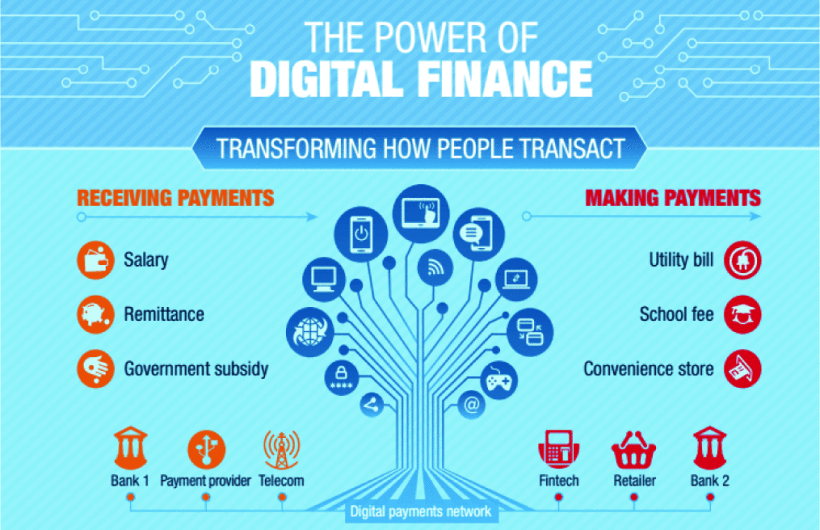
\includegraphics[width=0.90\textwidth]{src/resources/chapter-2-power-digital-finance.png}
    \caption{Transformasi Transaksi Finansial \textit{Fraud Detection System} \citep{8776857}}
    \label{fig:digital-finance}
\end{figure}

\vspace{10pt}

\subsection{Dasar Teori ke-4}

\blindtext

\blindtext

    %--------------------------------------------------------------------%
%
% Title         : Postgraduate Thesis LaTex template
% Author        : Ravi Vendra Rishika <ravi.vendra.rishika@gmail.com>
%
% Page          : Chapter 3
%
% It is developed especially for postgraduate students of :
%   Department of Informatics
%   Faculty of Intelligent Electrical and Informatics Technology
%   Institut Teknologi Sepuluh Nopember (ITS)
%   Surabaya, Indonesia.
%
% This LaTex template is intended to make students easier
% to write master's degree thesis in LaTex using specific
% Department of Informatics of ITS' format.
%
%--------------------------------------------------------------------%

\chapter{METODOLOGI PENELITIAN}

Bab 3 merupakan penjelasan terkait metodologi penelitian yang digunakan
dalam penelitian ini, yang terdiri dari empat tahapan, yakni tahap pertama diawali dengan melakukan studi literatur terlebih dahulu. Tahap kedua adalah perancangan metode yang digunakan dalam penelitian. Tahap ketiga adalah implementasi metode, uji coba dan analisis hasil. Selanjutnya, tahap terakhir adalah penyusunan laporan penelitian.

Penjelasan detail terkait setiap bagian dari alur penelitian akan dijelaskan secara komprehensif pada subbab berikut ini.

\section{Studi Literatur}

\blindtext

\section{Perancangan Metode}

\blindtext

\section{Penyusunan Laporan Penelitian}

\blindtext

    %--------------------------------------------------------------------%
%
% Title         : Postgraduate Thesis LaTex template
% Author        : Ravi Vendra Rishika <ravi.vendra.rishika@gmail.com>
%
% Page          : Chapter 4
%
% It is developed especially for postgraduate students of :
%   Department of Informatics
%   Faculty of Intelligent Electrical and Informatics Technology
%   Institut Teknologi Sepuluh Nopember (ITS)
%   Surabaya, Indonesia.
%
% This LaTex template is intended to make students easier
% to write master's degree thesis in LaTex using specific
% Department of Informatics of ITS' format.
%
%--------------------------------------------------------------------%

\chapter{EVALUASI DAN PEMBAHASAN}

\section{Tujuan Pengujian}

\blindtext

\section{Skenario Pengujian}

\blindtext

\section{Hasil Pengujian}

\blindtext

\section{Pembahasan}

\blindtext

    %--------------------------------------------------------------------%
%
% Title         : Postgraduate Thesis LaTex template
% Author        : Ravi Vendra Rishika <ravi.vendra.rishika@gmail.com>
%
% Page          : Chapter 5
%
% It is developed especially for postgraduate students of :
%   Department of Informatics
%   Faculty of Intelligent Electrical and Informatics Technology
%   Institut Teknologi Sepuluh Nopember (ITS)
%   Surabaya, Indonesia.
%
% This LaTex template is intended to make students easier
% to write master's degree thesis in LaTex using specific
% Department of Informatics of ITS' format.
%
%--------------------------------------------------------------------%

\chapter{PENUTUP}

\blindtext

\section{Kesimpulan}

\blindtext

\section{Saran}

\blindtext


    % Bibliography
    %--------------------------------------------------------------------%
%
% Title         : Postgraduate Thesis LaTex template
% Author        : Ravi Vendra Rishika <6025211015@mhs.its.ac.id>
%
% Page          : Bibliography
%
% It is developed especially for postgraduate students of :
%   Department of Informatics
%   Faculty of Intelligent Electrical and Informatics Technology
%   Institut Teknologi Sepuluh Nopember (ITS)
%   Surabaya, Indonesia.
%
% This LaTex template is intended to make students easier
% to write master's degree thesis in LaTex using specific
% Department of Informatics of ITS' format.
%
%--------------------------------------------------------------------%

\clearpage

% List of Bibliography
\addcontentsline{toc}{chapter}{Daftar Pustaka}

\bibliography{bibliography}

\printbibliography


    % Indexes
    % \appendix

    % \addcontentsline{toc}{part}{Lampiran}
    % \part*{Lampiran}

    % %--------------------------------------------------------------------%
%
% Title         : Postgraduate Thesis LaTex template
% Author        : Ravi Vendra Rishika <ravi.vendra.rishika@gmail.com>
%
% Page          : Appendix 1
%
% It is developed especially for postgraduate students of :
%   Department of Informatics
%   Faculty of Intelligent Electrical and Informatics Technology
%   Institut Teknologi Sepuluh Nopember (ITS)
%   Surabaya, Indonesia.
%
% This LaTex template is intended to make students easier
% to write master's degree thesis in LaTex using specific
% Department of Informatics of ITS' format.
%
%--------------------------------------------------------------------%

\clearpage

% List of Appendix 1
\addcontentsline{toc}{chapter}

\chapter{Instrumen Pengujian}

    % %--------------------------------------------------------------------%
%
% Title         : Postgraduate Thesis LaTex template
% Author        : Ravi Vendra Rishika <6025211015@mhs.its.ac.id>
%
% Page          : Appendix 2
%
% It is developed especially for postgraduate students of :
%   Department of Informatics
%   Faculty of Intelligent Electrical and Informatics Technology
%   Institut Teknologi Sepuluh Nopember (ITS)
%   Surabaya, Indonesia.
%
% This LaTex template is intended to make students easier
% to write master's degree thesis in LaTex using specific
% Department of Informatics of ITS' format.
%
%--------------------------------------------------------------------%

\clearpage

% List of Appendix 2
\addcontentsline{toc}{chapter}

\chapter{Rincian Kasus Uji}

    % %--------------------------------------------------------------------%
%
% Title         : Postgraduate Thesis LaTex template
% Author        : Ravi Vendra Rishika <6025211015@mhs.its.ac.id>
%
% Page          : Appendix 3
%
% It is developed especially for postgraduate students of :
%   Department of Informatics
%   Faculty of Intelligent Electrical and Informatics Technology
%   Institut Teknologi Sepuluh Nopember (ITS)
%   Surabaya, Indonesia.
%
% This LaTex template is intended to make students easier
% to write master's degree thesis in LaTex using specific
% Department of Informatics of ITS' format.
%
%--------------------------------------------------------------------%

\clearpage

% List of Appendix 3
\addcontentsline{toc}{chapter}

\chapter{Penjelasan Hasil}


\end{document}
